%\documentclass[12pt]{article}

\questionheader{ex:s1.9}

%%%%%%%%%%%%%%%%%%
%\subsection*{\Conceptual}
%%%%%%%%%%%%%%%%%%


%%%%%%%%%%%%%%%%%%
\subsection*{\Procedural}
%%%%%%%%%%%%%%%%%%

%%%%%%%%%%%%%%%%%%
\subsection*{\Application}
%%%%%%%%%%%%%%%%%%


%%%%%%%%%%%%%%%%%%%%%%%%%%%
\begin{question}[M317 2010A] %3
Let $\vr(t) = x(t)\,\hi + y (t)\,\hj + z(t)\,\hk$ be the position 
of a particle at time $t$ . Suppose the motion of the particle satisfies 
the differential equation
$\difftwo{\vr}{t} = f (r) \vr$ 
where $r = |\vr|$ .
\begin{enumerate}[(a)]
\item
Suppose $f(r)$ is an arbitrary function of $r$ . Prove or disprove each 
of the following statements.
\begin{enumerate}[(i)]
\item
The motion of the particle is planar.
\item
The path of the particle sweeps out equal areas in equal times.
\end{enumerate}
\item
Find all forms of $f(r)$ for which the motion of the particle always lies 
on a straight line.
\item
Give a specific form of $f(r)$ for which the motion of the particle could 
lie on an ellipse.
\end{enumerate}
\end{question}

\begin{hint} 
(a) Review \S\eref{CLP317}{sec:central forces} of the CLP-4 text.

(b) Any straight line can be parametrized as $\vr(s) = \vr_0+\hat\vT\, s$.

(c) Review \S\eref{CLP317}{sec:planet} of the CLP-4 text.
\end{hint}

\begin{answer}
(a) See the solutions. 

(b) $f(r)=0$ for all $r\ge 0$.

(c) Any $f(r)$ which is a positive constant times $-\frac{1}{r^3}$ works.
\end{answer}

\begin{solution} (a)
Both (i) and (ii) were proven in \S\eref{CLP317}{sec:central forces} 
of the CLP-4 text. Here are those arguments.

Define
\begin{equation*}
\vOm(t) = \vr(t)\times\vv(t)
\end{equation*}
By the product rule,
\begin{equation*}
\diff{\vOm}{t}(t) =\diff{\ }{t}\big(\vr(t)\times\vv(t)\big)
=\vv(t)\times\vv(t) + \vr(t)\times\va(t)
=m\vr(t)\times f\big(r(t))\vr(t)\big)
=\vZero
\end{equation*}
So $\vOm(t)$ is in fact independent of $t$. It is a constant vector that
we'll just denote $\vOm$. 

As $\vr(t)\times\vv(t)=\vOm$, we have that
$\vr(t)$ is always perpendicular to $\vOm$ and
\begin{equation*}
\vr(t)\cdot\vOm =0
\end{equation*}
\begin{itemize}\itemsep1pt \parskip0pt \parsep0pt %\itemindent-15pt
\item[$\circ$]
If $\vOm\ne \vZero$, this is exactly the statement that $\vr(t)$ always 
lies in the plane through the origin with normal vector $\vOm$.
\item[$\circ$]
If $\vOm=\vZero$, then $\vr(t)$ is always parallel to $\vv(t)$ and there
is some function $\alpha(t)$ such that
\begin{equation*}
\diff{\vr}{t}(t) = \vv(t) = \alpha(t)\,\vr(t)
\end{equation*}
This is a first order, linear, ordinary differential equation that we can solve
by using an integrating factor. Set
\begin{equation*}
\beta(t) = \int_0^t\alpha(t)\ \dee{t}
\end{equation*}
Then
\begin{align*}
\diff{\vr}{t}(t) = \alpha(t)\,\vr(t)
&\iff e^{-\beta(t)} \diff{\vr}{t}(t) -\alpha(t)e^{-\beta(t)}\,\vr(t)=0\\
&\iff \diff{\ }{t}\big[e^{-\beta(t)}\vr(t)\big] = 0\\
&\iff e^{-\beta(t)}\vr(t) = \vr(0)\\
&\iff \vr(t) =  e^{\beta(t)}\vr(0)
\end{align*}
so that $\vr(t)$ lies on a line through the origin. This makes sense ---
the particle is always moving parallel to its radius vector.
\end{itemize}
This completes the verification that $\vr(t)$ lies in a plane.

Now we show that the radius vector $\vr(t)$ sweeps out equal areas in 
equal times. In other words, we now verify that the rate at which 
$\vr(t)$ sweeps out area is independent of time. To do so we rewrite the
statement that $|\vr(t)\times\vv(t)\big|$ is constant in polar coordinates.
Writing $\vr(t) = r(t)\hat\vr\big(\theta(t)\big)$ and then applying
Lemma \eref{CLP317}{lem:polar}.b of the CLP-4 text gives that
\begin{align*}
\text{constant} = \big|\vr\times\vv\big| 
   = \Big|r\hat\vr\times\Big(\diff{r}{t}\ \hat\vr 
             + r\ \diff{\theta}{t}\ \hat\vth\Big)\Big|
   =r^2\diff{\theta}{t}
\qquad\text{since}\quad |\hat\vr\times\hat\vr|=0,\ 
                        |\hat\vr\times\hat\vth|=1
\end{align*}
is constant. It now suffices to observe that $r(t)^2\diff{\theta}{t}(t)$ 
is exactly twice the rate at which $\vr(t)$ sweeps out area. To see this,
just look at the figure below. The shaded area is essentially a wedge of
a circular disk of radius $r$. (If $r(t)$ were independent of $t$, it would be exactly a wedge of a circular disk.) Its area is the 
fraction $\frac{\dee{\theta}}{2\pi}$ of the area of the full disk, which is
\begin{equation*}
\frac{\dee{\theta}}{2\pi}\ \pi r^2 = \frac{1}{2}r^2\,\dee{\theta}
\qquad\qquad\raisebox{-0.35\height}[42pt][20pt]{
                 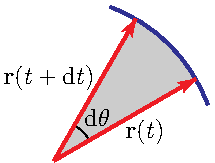
\includegraphics{fig/equalArea.pdf}}
\end{equation*}

\noindent (b) If $f(r)$ is identically zero, then $\vr''(t)=0$,
so that $\vr'(t)$ is a constant, say $\vv_0$, and $\vr(t) = \vr_0 + \vv_0 t$,
for some constant $\vr_0$. That's a straight line.

We'll now show that if the motion of the particle always lies 
on a straight line, then $f(r)$ must be identically zero.
Suppose that $\vr(t)$ is a straight line. Then there are 
constant vectors $\vr_0$ and $\hat\vT$ such that $\vr(t) =\vr_0+ g(t)\hat\vT$
for some scalar valued function $g(t)$. Then
\begin{align*}
\vr''(t) &= f\big(r(t)\big)\vr(t) \\
\end{align*}
becomes
\begin{align*}
g''(t)\hat\vT & = f\big(r(t)\big)\,\big[\vr_0+ g(t)\hat\vT\big]
              = f\big(r(t)\big)\,\vr_0
               + f\big(r(t)\big) g(t)\hat\vT
\end{align*}
We may always choose the initial conditions so that, for example, 
$\vr_0=\hi$ and $\hat\vT=\hj$.  So
\begin{align*}
g''(t)\hj &   = f\big(r(t)\big)\,\hi
               + f\big(r(t)\big) g(t)\hj
\end{align*}
Taking the dot product of both sides with $\hi$ gives 
$f\big(r(t)\big)=0$, as desired.


\noindent (c) We saw in \S\eref{CLP317}{sec:planet} of the CLP-4 text
that the gravitational force $-\frac{GMm}{r^3}\vr$ can produce 
elliptical orbits.
So any $f(r)$ which is a positive constant times $-\frac{1}{r^3}$ does 
the job. 

\end{solution}


%%%%%%%%%%%%%%%%%%%%%%%%%%%
\begin{question}[M317 2000A] %6
An object moves along a curve in the $xy$-plane having polar
equation $r=\frac{1}{\theta+\al}$ (where $\al$ is a constant) under the influence
of a central force so that the object has no transverse acceleration.
\begin{enumerate}[(a)]
\item
Verify that $r^2\dot\theta=h$ remains constant as the object
moves.
\item
Express the magnitude of the acceleration of the object as
a function of $r$ and $h$.
\end{enumerate}

\end{question}

\begin{hint} 
(a) For any central force $\big|\vr(t)\times\vv(t)\big|$ is independent of $t$.

(b) Review Lemma \eref{CLP317}{lem:polar} in the CLP-4 text.
\end{hint}

\begin{answer}
(a) See the solution.

(b) $|\va(t)| =\frac{h^2}{r(t)^3}$
\end{answer}

\begin{solution} 
(a)
Our object is subject to a central force. So the acceleration $\va(t)$
is parallel to $\vr(t)$ and
\begin{equation*}
\diff{\ }{t}\big(\vr(t)\times\vv(t)\big)
=\vv(t)\times\vv(t) + \vr(t)\times\va(t)
=\vZero +\vZero
=\vZero
\end{equation*}
By Lemma \eref{CLP317}{lem:polar} of the CLP-4 text,
$\vv(t) = \diff{r}{t}(t)\ \hat\vr\big(\theta(t)\big) 
             + r(t)\ \diff{\theta}{t}(t)\ \hat\vth\big(\theta(t)\big)$.
Because $\vr(t)=r(t)\hat\vr\big(\theta(t)\big)$ is parallel to 
$\hat\vr\big(\theta(t)\big)$ and is perpendicular to 
$\hat\vth\big(\theta(t)\big)$,
\begin{equation*}
\vr(t)\times\vv(t)
=r(t)^2\dot\theta(t)\,\hat\vr\big(\theta(t)\big)\times
                       \hat\vth\big(\theta(t)\big)
\end{equation*}
and, in particular,
\begin{equation*}
|\vr(t)\times\vv(t)| = r(t)^2|\dot\theta(t)|
\end{equation*}
is a constant. As $\dot\theta(t)$ is continuous, $r(t)^2\dot\theta(t)$
is also constant.

(b) 
By Lemma \eref{CLP317}{lem:polar} of the CLP-4 text,
the acceleration
\begin{equation*}
\va(t) = \Big(\difftwo{r}{t}(t)-r(t)\Big(\diff{\theta}{t}(t)\Big)^2\Big) 
             \hat\vr\big(\theta(t)\big)
   +\Big(r(t)\ \difftwo{\theta}{t}(t) 
          + 2 \diff{r}{t}(t)\diff{\theta}{t}(t)\Big)
                  \hat\vth\big(\theta(t)\big)
\end{equation*}
Because our object is subject to a central force, the acceleration 
$\va(t)$ is parallel to $\hat\vr\big(\theta(t)\big)$. So the 
$\hat\vth\big(\theta(t)\big)$ component of the acceleration is zero 
and
\begin{equation*}
\va(t) = \Big(\difftwo{r}{t}(t)-r(t)\Big(\diff{\theta}{t}(t)\Big)^2\Big) 
             \hat\vr\big(\theta(t)\big)
\end{equation*}
so that
\begin{equation*}
|\va(t)| = \Big|\difftwo{r}{t}(t)-r(t)\Big(\diff{\theta}{t}(t)\Big)^2\Big|
\end{equation*}
Since $r(t)=\frac{1}{\theta(t)+\al}$
\begin{align*}
\dot r(t) = - \frac{1}{[\theta(t)+\al]^2}\dot\theta(t)
          =- r(t)^2 \dot\theta(t) =-h
\end{align*}
So $\difftwo{r}{t}(t)=0$ and
\begin{align*}
|\va(t)| = r(t)\dot\theta(t)^2
=\frac{r(t)^4\dot\theta(t)^2}{r(t)^3}
=\frac{h^2}{r(t)^3}
\end{align*}

\end{solution}






